\subsection{Упражнение 1}

Скачайте с сайта http://freesound.org , включающий музыку, речь или иные звуки, имеющие четко выраженную высоту. Выделите примерно полусекундный сегмент, в котором высота постоянна. Вычислите и распечатайте спектр выбранного сегмента. Как связаны тембр звука и гармоническая структура, видимая в спектре?


\noindent Используйте high\_pass, low\_pass, и band\_stop для фильтрациитех или иных гармоник. Затем преобразуйте спектры обратно в сигнал и прослушайте его. Как звук соотносится с изменениями, сделанными в спектре?
    

Был выбран звук пианино, загружаем его, прослушиваем, затем вырезаем полусекундный фрагмент выбранного звука и строим wave график.

\begin{lstlisting}[language=Python]
if not os.path.exists('440931__xhale303__piano-loop-1.wav'):
    !wget https://github.com/Eugenepolyt/ThinkDSP/raw/master/440931__xhale303__piano-loop-1.wav
wave = read_wave('440931__xhale303__piano-loop-1.wav')
wave.make_audio()
segment = wave.segment(start=1.5, duration=0.5)
segment.make_audio()
segment.plot()
\end{lstlisting}
    
\begin{figure}[H]
	\begin{center}
		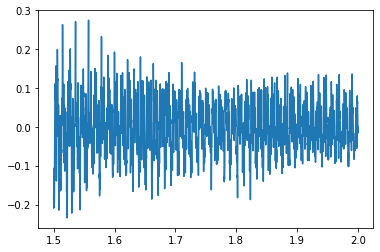
\includegraphics[scale=1]{fig/lab01/lab01_1.png}
		\caption{График выделенного сегмента}
	\end{center}
\end{figure}

Вычислим спектр выделенного сегмента и построим график.
\begin{lstlisting}[language=Python]
spectrum = segment.make_spectrum()
spectrum.plot(high=3000)
decorate(xlabel='Frequency')
\end{lstlisting}

\begin{figure}[H]
	\begin{center}
		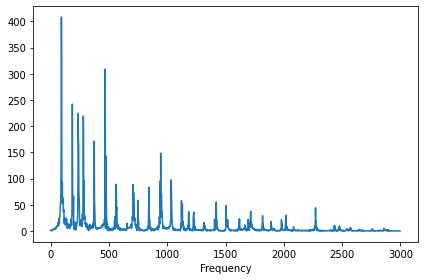
\includegraphics[scale=1]{fig/lab01/lab01_2.png}
		\caption{Спектр звука фрагмента}
	\end{center}
\end{figure}

В данном примере основная частота является доминирующей, воспринимаемая высота звука сильно зависит от основной частоты. Используем функции для фильтрации для данного спектра.


Уберем частоты выше 1500.

\begin{lstlisting}[language=Python]
spectrum.low_pass(1500)
spectrum.plot(high=3000)
decorate(xlabel='Frequency')
\end{lstlisting}

\begin{figure}[H]
	\begin{center}
		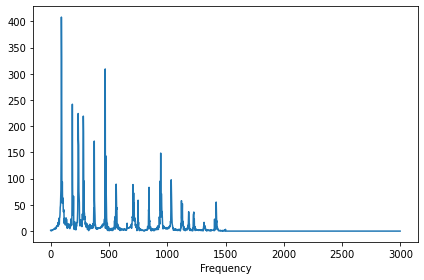
\includegraphics[scale=1]{fig/lab01/lab01_3.png}
		\caption{Спектр звука c урезанными частотами}
	\end{center}
\end{figure}

Уберем частоты ниже 400, тем самым изменим доминирующую частоту.

\begin{figure}[H]
	\begin{center}
		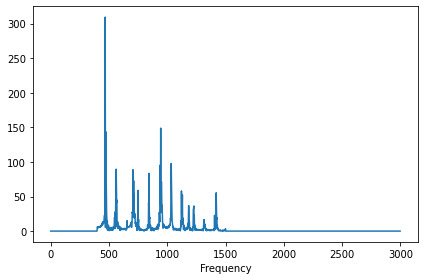
\includegraphics[scale=1]{fig/lab01/lab01_4.png}
		\caption{Спектр звука c частотами выше 400 и ниже 1500}
	\end{center}
\end{figure}

Применим ФПЗ.

\begin{lstlisting}[language=Python]
spectrum.band_stop(500, 800)
spectrum.plot(high=3000)
decorate(xlabel='Frequency')
\end{lstlisting}

\begin{figure}[H]
	\begin{center}
		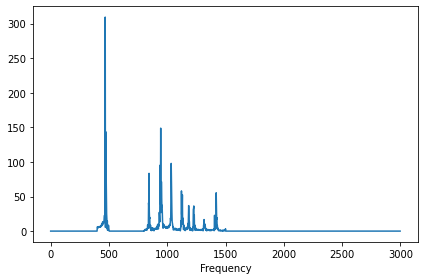
\includegraphics[scale=1]{fig/lab01/lab01_5.png}
		\caption{Спектр звука после ФПЗ}
	\end{center}
\end{figure}

Преобразуем спектр обратно в сигнал.

\begin{lstlisting}[language=Python]
filtered = spectrum.make_wave()
filtered.plot()
decorate(xlabel='Time')
\end{lstlisting}

Сравниваем первоначальный сигнал с отфильтрованным фрагментом.

\begin{lstlisting}[language=Python]
segment.make_audio()
filtered.make_audio()
\end{lstlisting}

После обработки звук звучит уже не так объемно, и напоминает гудок, а не пианино

\subsection{Упражнение 2}

Создайте сложный сигнал из объектов SinSignal и CosSignal, суммируя их. Обработайте сигнал для получения wave и прослушайте его. Вычислите Spectrum и распечатайте. Что произойдёт при добавлении частотных компонент, не кратных основным?


Создадим сложный сигнал из CosSignal и SinSignal и построим график.
\begin{lstlisting}[language=Python]
cos_sig = CosSignal(freq=50, amp=0.8, offset=0)
sin_sig = SinSignal(freq=200, amp=0.4, offset=0)
cos2_sig = SinSignal(freq=600, amp=0.6, offset=0)
sin2_sig = SinSignal(freq=1000, amp=0.2, offset=0)
m_sig = cos_sig + sin_sig + sin2_sig + cos2_sig
\end{lstlisting}

\begin{figure}[H]
	\begin{center}
		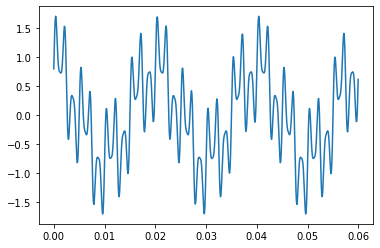
\includegraphics[scale=1]{fig/lab01/lab01_6.png}
		\caption{Граффик после суммирования сигналов}
	\end{center}
\end{figure}

Создадим wave и вычислим спектр.

\begin{lstlisting}[language=Python]
wave = m_sig.make_wave()
wave.make_audio()
spectrum = wave.make_spectrum()
spectrum.plot()
\end{lstlisting}

\begin{figure}[H]
	\begin{center}
		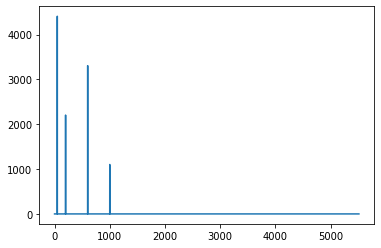
\includegraphics[scale=1]{fig/lab01/lab01_7.png}
		\caption{Спектр сигнала}
	\end{center}
\end{figure}

Добавим частотный компонент, не кратный основным.

\begin{lstlisting}[language=Python]
secondWave = (m_sig + CosSignal(freq=440, amp=0.75, offset=0)).make_wave()
secondWave.make_audio()
spectr = secondWave.make_spectrum()
spectr.plot()
\end{lstlisting}

\begin{figure}[H]
	\begin{center}
		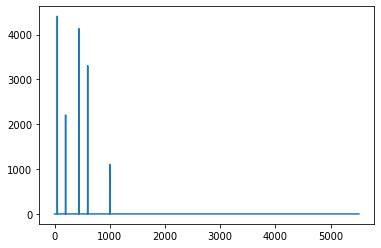
\includegraphics[scale=1]{fig/lab01/lab01_8.png}
		\caption{Спектр после изменения}
	\end{center}
\end{figure}

После изменения звук стал не таким однотонным, каким был. 


\subsection{Упражнение 3}

Напишите функцию strech, берущую wave и коэффицент изменения. Она должна ускорять или замедлять сигнал изменением ts и framerate.

Напишем необходимую функцию.

\begin{lstlisting}[language=Python]
def stretch(wave, coef):
  wave.ts *= coef
  wave.framerate /= coef
\end{lstlisting}

\begin{figure}[H]
	\begin{center}
		
\includegraphics[scale=1]{fig/lab01/lab01_9.png}
		\caption{Длинна изначального звука пианино}
	\end{center}
\end{figure}

Попробуем ускорить и замедлить звук пианино.

\begin{lstlisting}[language=Python]
fasterX2 = wave
stretch(fasterX2, 0.5)
fasterX2.make_audio()

slowX2 = read_wave('440931__xhale303__piano-loop-1.wav')
stretch(slowX2, 2)
slowX2.make_audio()
\end{lstlisting}

\begin{figure}[H]
	\begin{center}
		
\includegraphics[scale=1]{fig/lab01/lab01_10.png}
		\caption{Длинна ускоренного звука}
	\end{center}
\end{figure}

\begin{figure}[H]
	\begin{center}
		
\includegraphics[scale=1]{fig/lab01/lab01_11.png}
		\caption{Длинна замедленного звука}
	\end{center}
\end{figure}

По рисункам можно заметить , что функция работает весьма успешно, в случае ускорения длинна дорожки сокращается в два раза, в случае замедленния, увеличивается в два раза.



\subsection{Вывод}
В данной лабораторной работе, были изучены основные понятия при работе со звуком и проведена работа с библиотекой thinkDSP, которая позваляет производить различные действия с сигналами.